\section{Register description}
\regover{
{\hyperref[dbi-dbi-config]{dbi\_config}}&
\\
\hline
{\hyperref[dbi-dbi-int-sts]{dbi\_int\_sts}}&
\\
\hline
{\hyperref[dbi-dbi-bus-busy]{dbi\_bus\_busy}}&
\\
\hline
{\hyperref[dbi-dbi-pix-cnt]{dbi\_pix\_cnt}}&
\\
\hline
{\hyperref[dbi-dbi-prd]{dbi\_prd}}&
\\
\hline
{\hyperref[dbi-dbi-wdata]{dbi\_wdata}}&
\\
\hline
{\hyperref[dbi-dbi-rdata]{dbi\_rdata}}&
\\
\hline
{\hyperref[dbi-dbi-fifo-config-0]{dbi\_fifo\_config\_0}}&
\\
\hline
{\hyperref[dbi-dbi-fifo-config-1]{dbi\_fifo\_config\_1}}&
\\
\hline
{\hyperref[dbi-dbi-fifo-wdata]{dbi\_fifo\_wdata}}&
\\
\hline
}

\subsection{dbi\_config}
\label{dbi-dbi-config}
Address:0x3001b000
 \begin{figure}[H]
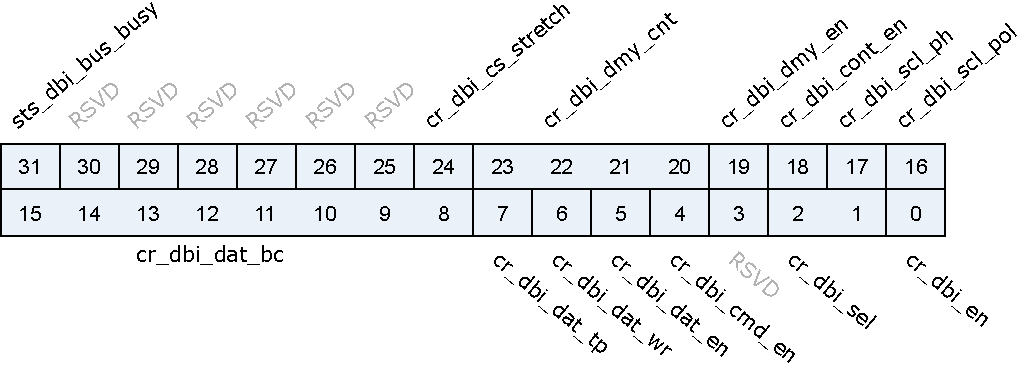
\includegraphics{dbi_dbi_config.pdf}
\end{figure}

\regdes{31:29&cr\_dbi\_tc\_deg\_cnt&r/w&3'd0&De-glitch function cycle count\\\hline
28&cr\_dbi\_tc\_deg\_en&r/w&1'b0&Enable signal of all input de-glitch function\\\hline
27&cr\_dbi\_tc\_3w\_mode&r/w&1'b0&DBI Type C 3-wire mode enable \par 1'b0: 4-wire mode is enabled \par 1'b1: 3-wire mode is enabled
\\\hline
26:24&rsvd&rsvd&3'h0&\\\hline
23:20&cr\_dbi\_dmy\_cnt&r/w&4'd0&Dummy cycle count, unit: period defined by dbi\_prd\_d \par Effective only in Type C (Fixed to 1 dbi\_prd\_d  period in Type B)
\\\hline
19&cr\_dbi\_dmy\_en&r/w&1'b0&Enable signal of dummy cycle(s) \par 1'b0: Disabled, no dummy cycle(s) between command phase and data phase \par 1'b1: Enabled, dummy cycle(s) will be inserted between command phase and data phase
\\\hline
18&cr\_dbi\_cont\_en&r/w&1'b1&Enable signal of pixel data continuous transfer mode \par 1'b0: Disabled, CS\_n will de-assert between each pixel \par 1'b1: Enabled, CS\_n will stay asserted between each consecutive pixel
\\\hline
17&cr\_dbi\_scl\_ph&r/w&1'b0&SCL clock phase inverse signal\\\hline
16&cr\_dbi\_scl\_pol&r/w&1'b1&SCL clock polarity \par 0: SCL output LOW at IDLE state \par 1: SCL output HIGH at IDLE state
\\\hline
15:8&cr\_dbi\_cmd&r/w&8'h2C&DBI Command\\\hline
7:6&cr\_dbi\_dat\_bc&r/w&2'd0&Data byte count of normal data (pixel data count is determined by cr\_dbi\_pix\_cnt)\\\hline
5&cr\_dbi\_dat\_tp&r/w&1'b0&Data type select \par 1'b0: Normal data (parameter) \par 1'b1: Pixel data \par Note: Read command supports normal data only
\\\hline
4&cr\_dbi\_dat\_wr&r/w&1'b1&Data phase Read/Write select \par 1'b0: Read data \par 1'b1: Write data
\\\hline
3&cr\_dbi\_dat\_en&r/w&1'b1&Data enable signal \par 1'b0: Data phase disabled \par 1'b1: Data phase enabled
\\\hline
2&cr\_dbi\_cmd\_en&r/w&1'b1&Command enable signal \par 1'b0: No command phase \par 1'b1: Command will be sent
\\\hline
1&cr\_dbi\_sel&r/w&1'b0&Select signal of DBI Type B or C \par 1'b0: DBI Type B \par 1'b1: DBI Type C
\\\hline
0&cr\_dbi\_en&r/w&1'b0&Enable signal of DBI function \par Asserting this bit will trigger the transaction, and should be de-asserted after finish
\\\hline

}
\subsection{dbi\_int\_sts}
\label{dbi-dbi-int-sts}
Address:0x3001b004
 \begin{figure}[H]
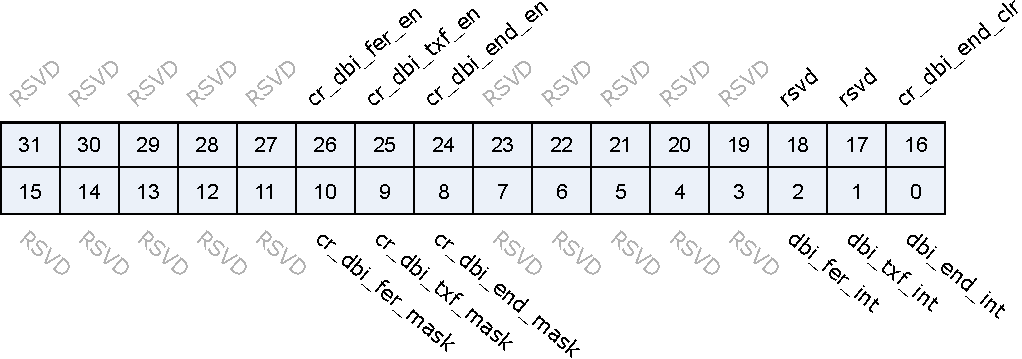
\includegraphics{dbi_dbi_int_sts.pdf}
\end{figure}

\regdes{31:27&RSVD& & & \\\hline
26&cr\_dbi\_fer\_en&r/w&1'b1&Interrupt enable of dbi\_fer\_int\\\hline
25&cr\_dbi\_txf\_en&r/w&1'b1&Interrupt enable of dbi\_txe\_int\\\hline
24&cr\_dbi\_end\_en&r/w&1'b1&Interrupt enable of dbi\_end\_int\\\hline
23:19&RSVD& & & \\\hline
18&rsvd&rsvd&1'b0&\\\hline
17&rsvd&rsvd&1'b0&\\\hline
16&cr\_dbi\_end\_clr&w1c&1'b0&Interrupt clear of dbi\_end\_int\\\hline
15:11&RSVD& & & \\\hline
10&cr\_dbi\_fer\_mask&r/w&1'b1&Interrupt mask of dbi\_fer\_int\\\hline
9&cr\_dbi\_txf\_mask&r/w&1'b1&Interrupt mask of dbi\_txe\_int\\\hline
8&cr\_dbi\_end\_mask&r/w&1'b1&Interrupt mask of dbi\_end\_int\\\hline
7:3&RSVD& & & \\\hline
2&dbi\_fer\_int&r&1'b0&TX/RX FIFO error interrupt, auto-cleared when FIFO overflow/underflow error flag is cleared\\\hline
1&dbi\_txf\_int&r&1'b1&TX FIFO ready (tx\_fifo\_cnt > tx\_fifo\_th) interrupt, auto-cleared when data is pushed\\\hline
0&dbi\_end\_int&r&1'b0&Transfer end interrupt, shared by both Type B and C mode\\\hline

}
\subsection{dbi\_bus\_busy}
\label{dbi-dbi-bus-busy}
Address:0x3001b008
 \begin{figure}[H]
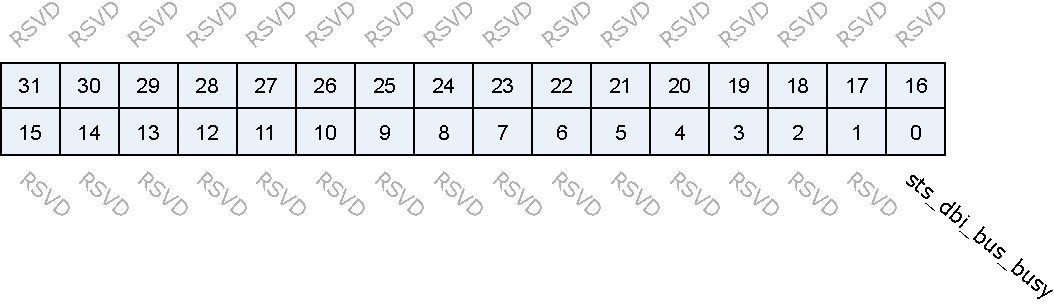
\includegraphics{dbi_dbi_bus_busy.pdf}
\end{figure}

\regdes{31:1&RSVD& & & \\\hline
0&sts\_dbi\_bus\_busy&r&1'b0&Indicator of dbi bus busy\\\hline

}
\subsection{dbi\_pix\_cnt}
\label{dbi-dbi-pix-cnt}
Address:0x3001b00c
 \begin{figure}[H]
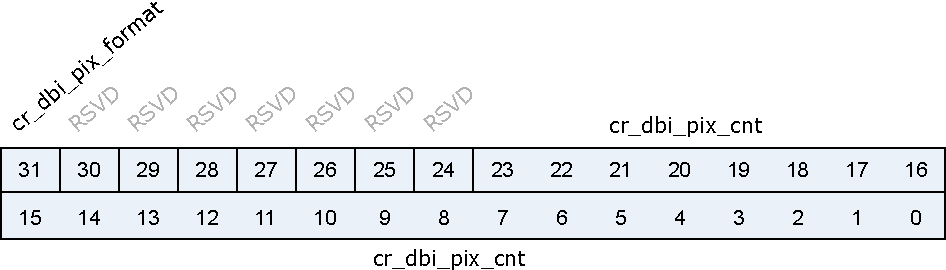
\includegraphics{dbi_dbi_pix_cnt.pdf}
\end{figure}

\regdes{31&cr\_dbi\_pix\_format&r/w&1'b0&Pixel format \par 1'b0: RGB565 \par 1'b1: RGB888/RGB666
\\\hline
30:24&RSVD& & & \\\hline
23:0&cr\_dbi\_pix\_cnt&r/w&24'h0&Pixel count\\\hline

}
\subsection{dbi\_prd}
\label{dbi-dbi-prd}
Address:0x3001b010
 \begin{figure}[H]
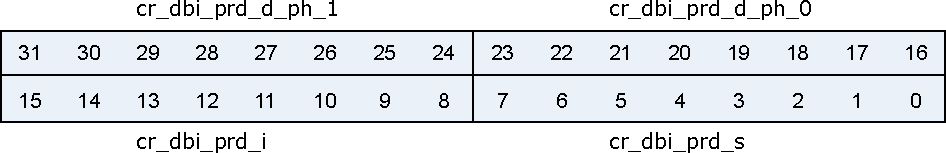
\includegraphics{dbi_dbi_prd.pdf}
\end{figure}

\regdes{31:24&cr\_dbi\_prd\_d\_ph\_1&r/w&8'd15&Length of DATA phase 1 (please refer to "Timing" tab)\\\hline
23:16&cr\_dbi\_prd\_d\_ph\_0&r/w&8'd15&Length of DATA phase 0 (please refer to "Timing" tab)\\\hline
15:8&cr\_dbi\_prd\_i&r/w&8'd15&Length of INTERVAL between pixel data (please refer to "Timing" tab)\\\hline
7:0&cr\_dbi\_prd\_s&r/w&8'd15&Length of START/STOP condition (please refer to "Timing" tab)\\\hline

}
\subsection{dbi\_wdata}
\label{dbi-dbi-wdata}
Address:0x3001b018
 \begin{figure}[H]
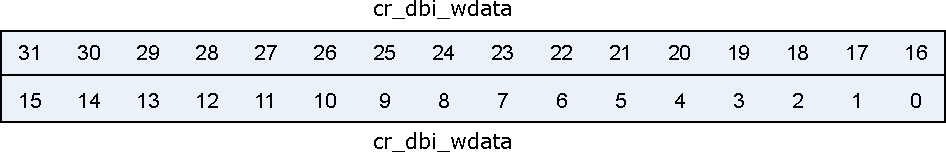
\includegraphics{dbi_dbi_wdata.pdf}
\end{figure}

\regdes{31:0&cr\_dbi\_wdata&r/w&32'h0&Data to be written into display IC using write command\\\hline

}
\subsection{dbi\_rdata}
\label{dbi-dbi-rdata}
Address:0x3001b01c
 \begin{figure}[H]
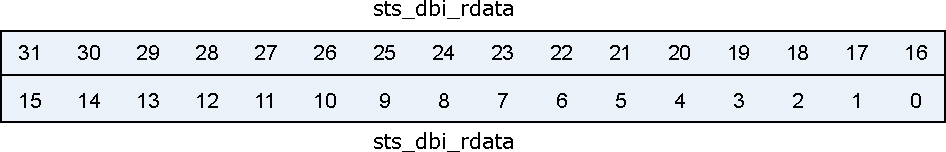
\includegraphics{dbi_dbi_rdata.pdf}
\end{figure}

\regdes{31:0&sts\_dbi\_rdata&r&32'h0&Data read from display IC using read command\\\hline

}
\subsection{dbi\_fifo\_config\_0}
\label{dbi-dbi-fifo-config-0}
Address:0x3001b080
 \begin{figure}[H]
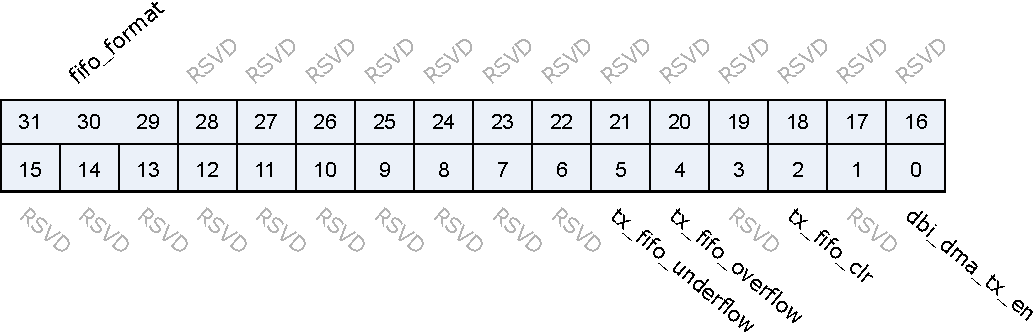
\includegraphics{dbi_dbi_fifo_config_0.pdf}
\end{figure}

\regdes{31:29&fifo\_format&r/w&3'd0&FIFO data format (see Tab 'FIFO Format' for details) \par 3'd0: {8'h0, B[7:0], G[7:0], R[7:0]} \par 3'd1: {8'h0, R[7:0], G[7:0], B[7:0]} \par 3'd2: {B[7:0], G[7:0], R[7:0], 8'h0} \par 3'd3: {R[7:0], G[7:0], B[7:0], 8'h0} \par 3'd4: {R[7:0], B[7:0], G[7:0], R[7:0]} \par 3'd5: {B[7:0], R[7:0], G[7:0], B[7:0]} \par 3'd6: {2{B[7:3], G[7:2], R[7:3]}} \par 3'd7: {2{R[7:3], G[7:2], B[7:3]}}
\\\hline
28:6&RSVD& & & \\\hline
5&tx\_fifo\_underflow&r&1'b0&Underflow flag of TX FIFO, can be cleared by tx\_fifo\_clr\\\hline
4&tx\_fifo\_overflow&r&1'b0&Overflow flag of TX FIFO, can be cleared by tx\_fifo\_clr\\\hline
3&RSVD& & & \\\hline
2&tx\_fifo\_clr&w1c&1'b0&Clear signal of TX FIFO\\\hline
1&RSVD& & & \\\hline
0&dbi\_dma\_tx\_en&r/w&1'b0&Enable signal of dma\_tx\_req/ack interface\\\hline

}
\subsection{dbi\_fifo\_config\_1}
\label{dbi-dbi-fifo-config-1}
Address:0x3001b084
 \begin{figure}[H]
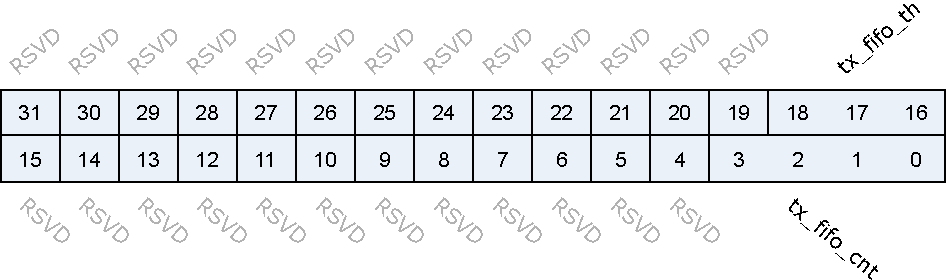
\includegraphics{dbi_dbi_fifo_config_1.pdf}
\end{figure}

\regdes{31:19&RSVD& & & \\\hline
18:16&tx\_fifo\_th&r/w&3'd0&TX FIFO threshold, dma\_tx\_req will not be asserted if tx\_fifo\_cnt is less than this value\\\hline
15:4&RSVD& & & \\\hline
3:0&tx\_fifo\_cnt&r&4'd8&TX FIFO available count\\\hline

}
\subsection{dbi\_fifo\_wdata}
\label{dbi-dbi-fifo-wdata}
Address:0x3001b088
 \begin{figure}[H]
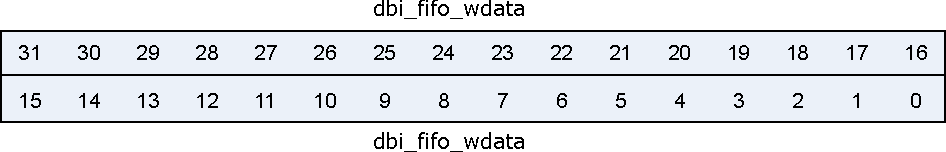
\includegraphics{dbi_dbi_fifo_wdata.pdf}
\end{figure}

\regdes{31:0&dbi\_fifo\_wdata&w&x&Pixel data with 8 types of format (determined by fifo\_format)\\\hline

}
